\documentclass{article}
\usepackage{amsmath}
\usepackage{amsfonts}
\usepackage{amssymb}
\usepackage{graphicx}
\usepackage{cancel}

\setlength\parindent{0pt}

\author{Pranav Tikkawar}
\title{Workshop 2}
\begin{document}
\maketitle
1. How Much to fish? \\
(a)  \begin{itemize}
    \item The IVP that models this relation is$y'(t) = k y(t) - c $ 
    \item Where $y(t_0) = y_0 $ is the intial condition
\end{itemize}
(b) \begin{itemize}
    \item The process of solving this IVP is to use an integrating factor $h(t)$ to multiply through the DE and then "group" the left side as the derivative of the product of 2 functions
    \item $y' - ky = -c $ 
    \item $h(t) = e^{-kt} $
    \item $h'(t) = -ke^{-kt} = -k h(t) $
    \item $hy' - khy = -ch $
    \item $[h(t)y(t)]' = -ch(t) $
    \item $h(t)y(t) - h(t_0)y_0 = -c\int_{t_0}^{t}h(t)dt$
    \item After simplifying and replacing $h(t)$, $h'(t)$ we get:
    \item $y(t) = y_0 e^{kt} + c(\frac{1}{k} - \frac{e^{kt}}{k})$
    \item k is $\frac{ln(2)}{5}$ as we know the populaiton doubles every 5 weeks. 
    \item so $y(t) = y_0 e^{\frac{ln(2)}{5}t} + c(\frac{5}{ln(2)} - \frac{5e^{\frac{ln(2)}{5}t}}{ln(2)}) $
\end{itemize}
(c)\begin{itemize}
    \item as $t \rightarrow \infty ; y(t) \rightarrow -\infty$
    \item See image at bottom
\end{itemize}
(d) \begin{itemize}
    \item c would be ln(2)/5 as that would lead the the funciton y(t) = 1 for all values of t
\end{itemize} 
(e) \begin{itemize}
    \item $ \Phi_{t,0}(y)= ye^{\frac{ln(2)}{5}t} + c(\frac{5}{ln(2)} - \frac{5e^{\frac{ln(2)}{5}t}}{ln(2)}) $
    \item We replace the $y_0$ for $y $
\end{itemize}
\begin{center}
    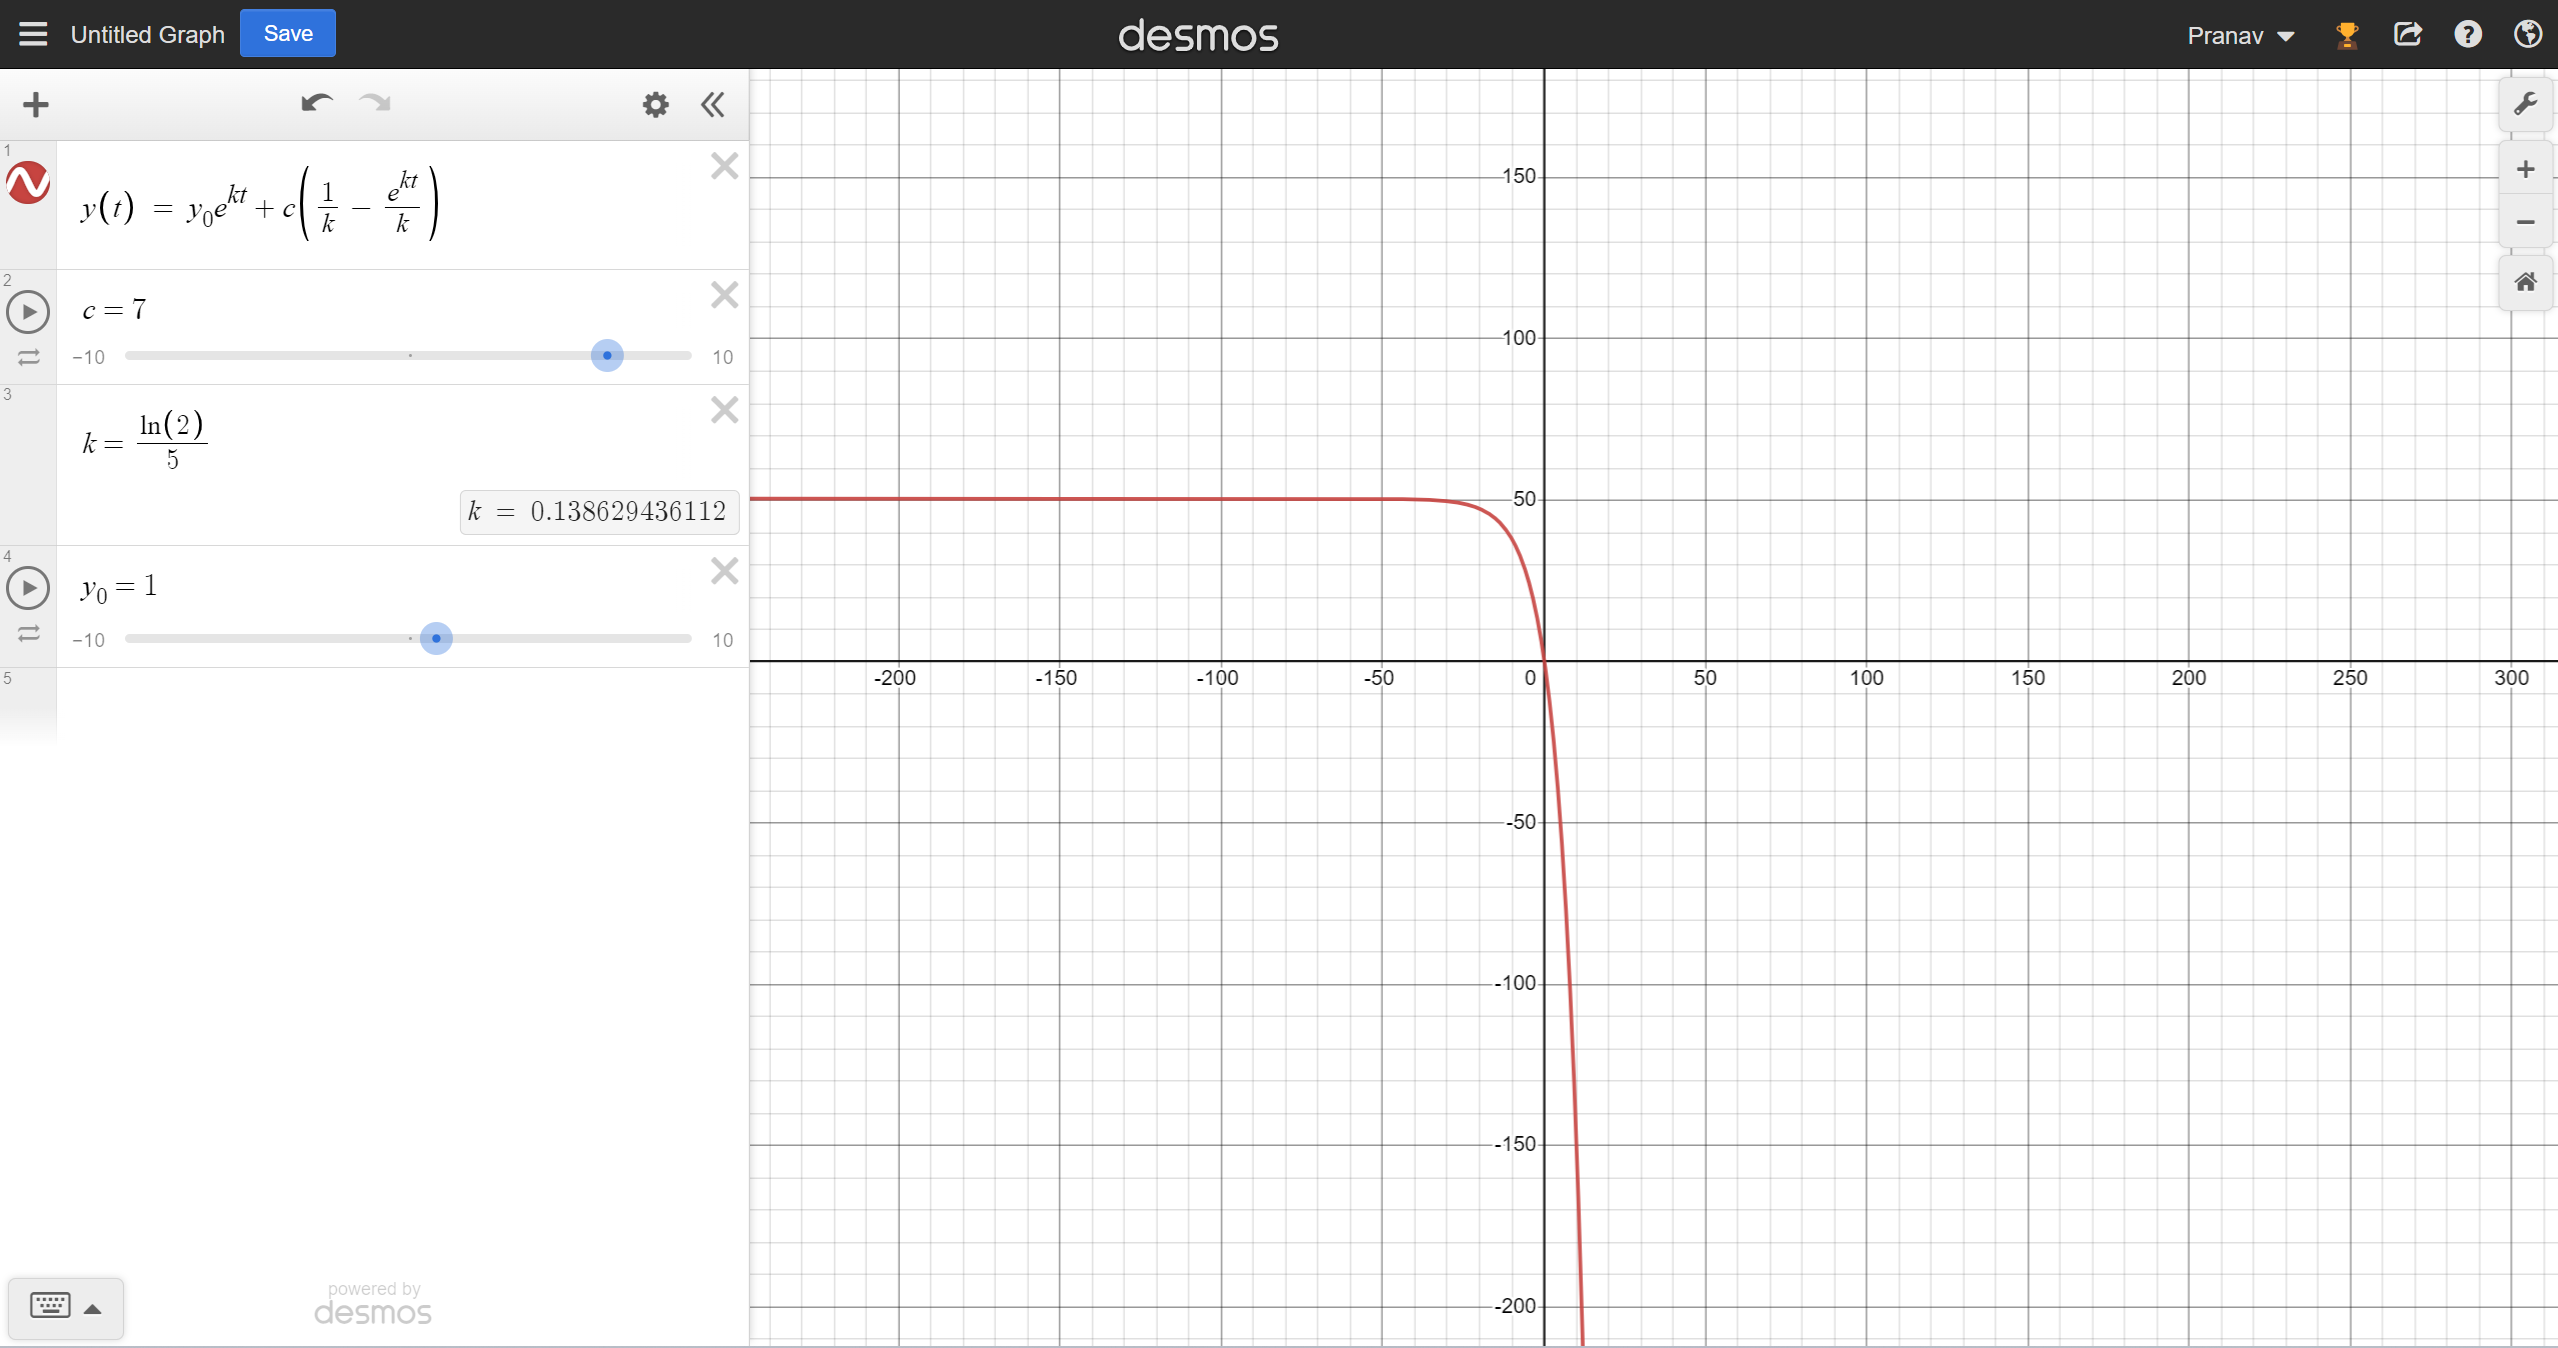
\includegraphics[scale=.2]{FishPlot.png}
\end{center}


\end{document}

